%!TEX program = xelatex
\documentclass[12pt]{beamer}

%\usepackage{multimedia}
%\usepackage{hyperref}
\usepackage{media9}

%% Title
\author{\textbf{Andrew Dixon} \\ Supervisor: Dr Panagiotis (Takis) Tsoutsanis \\ } 
\title{\LARGE Traffic Flow Modelling}
\subtitle{\vspace{0.4cm}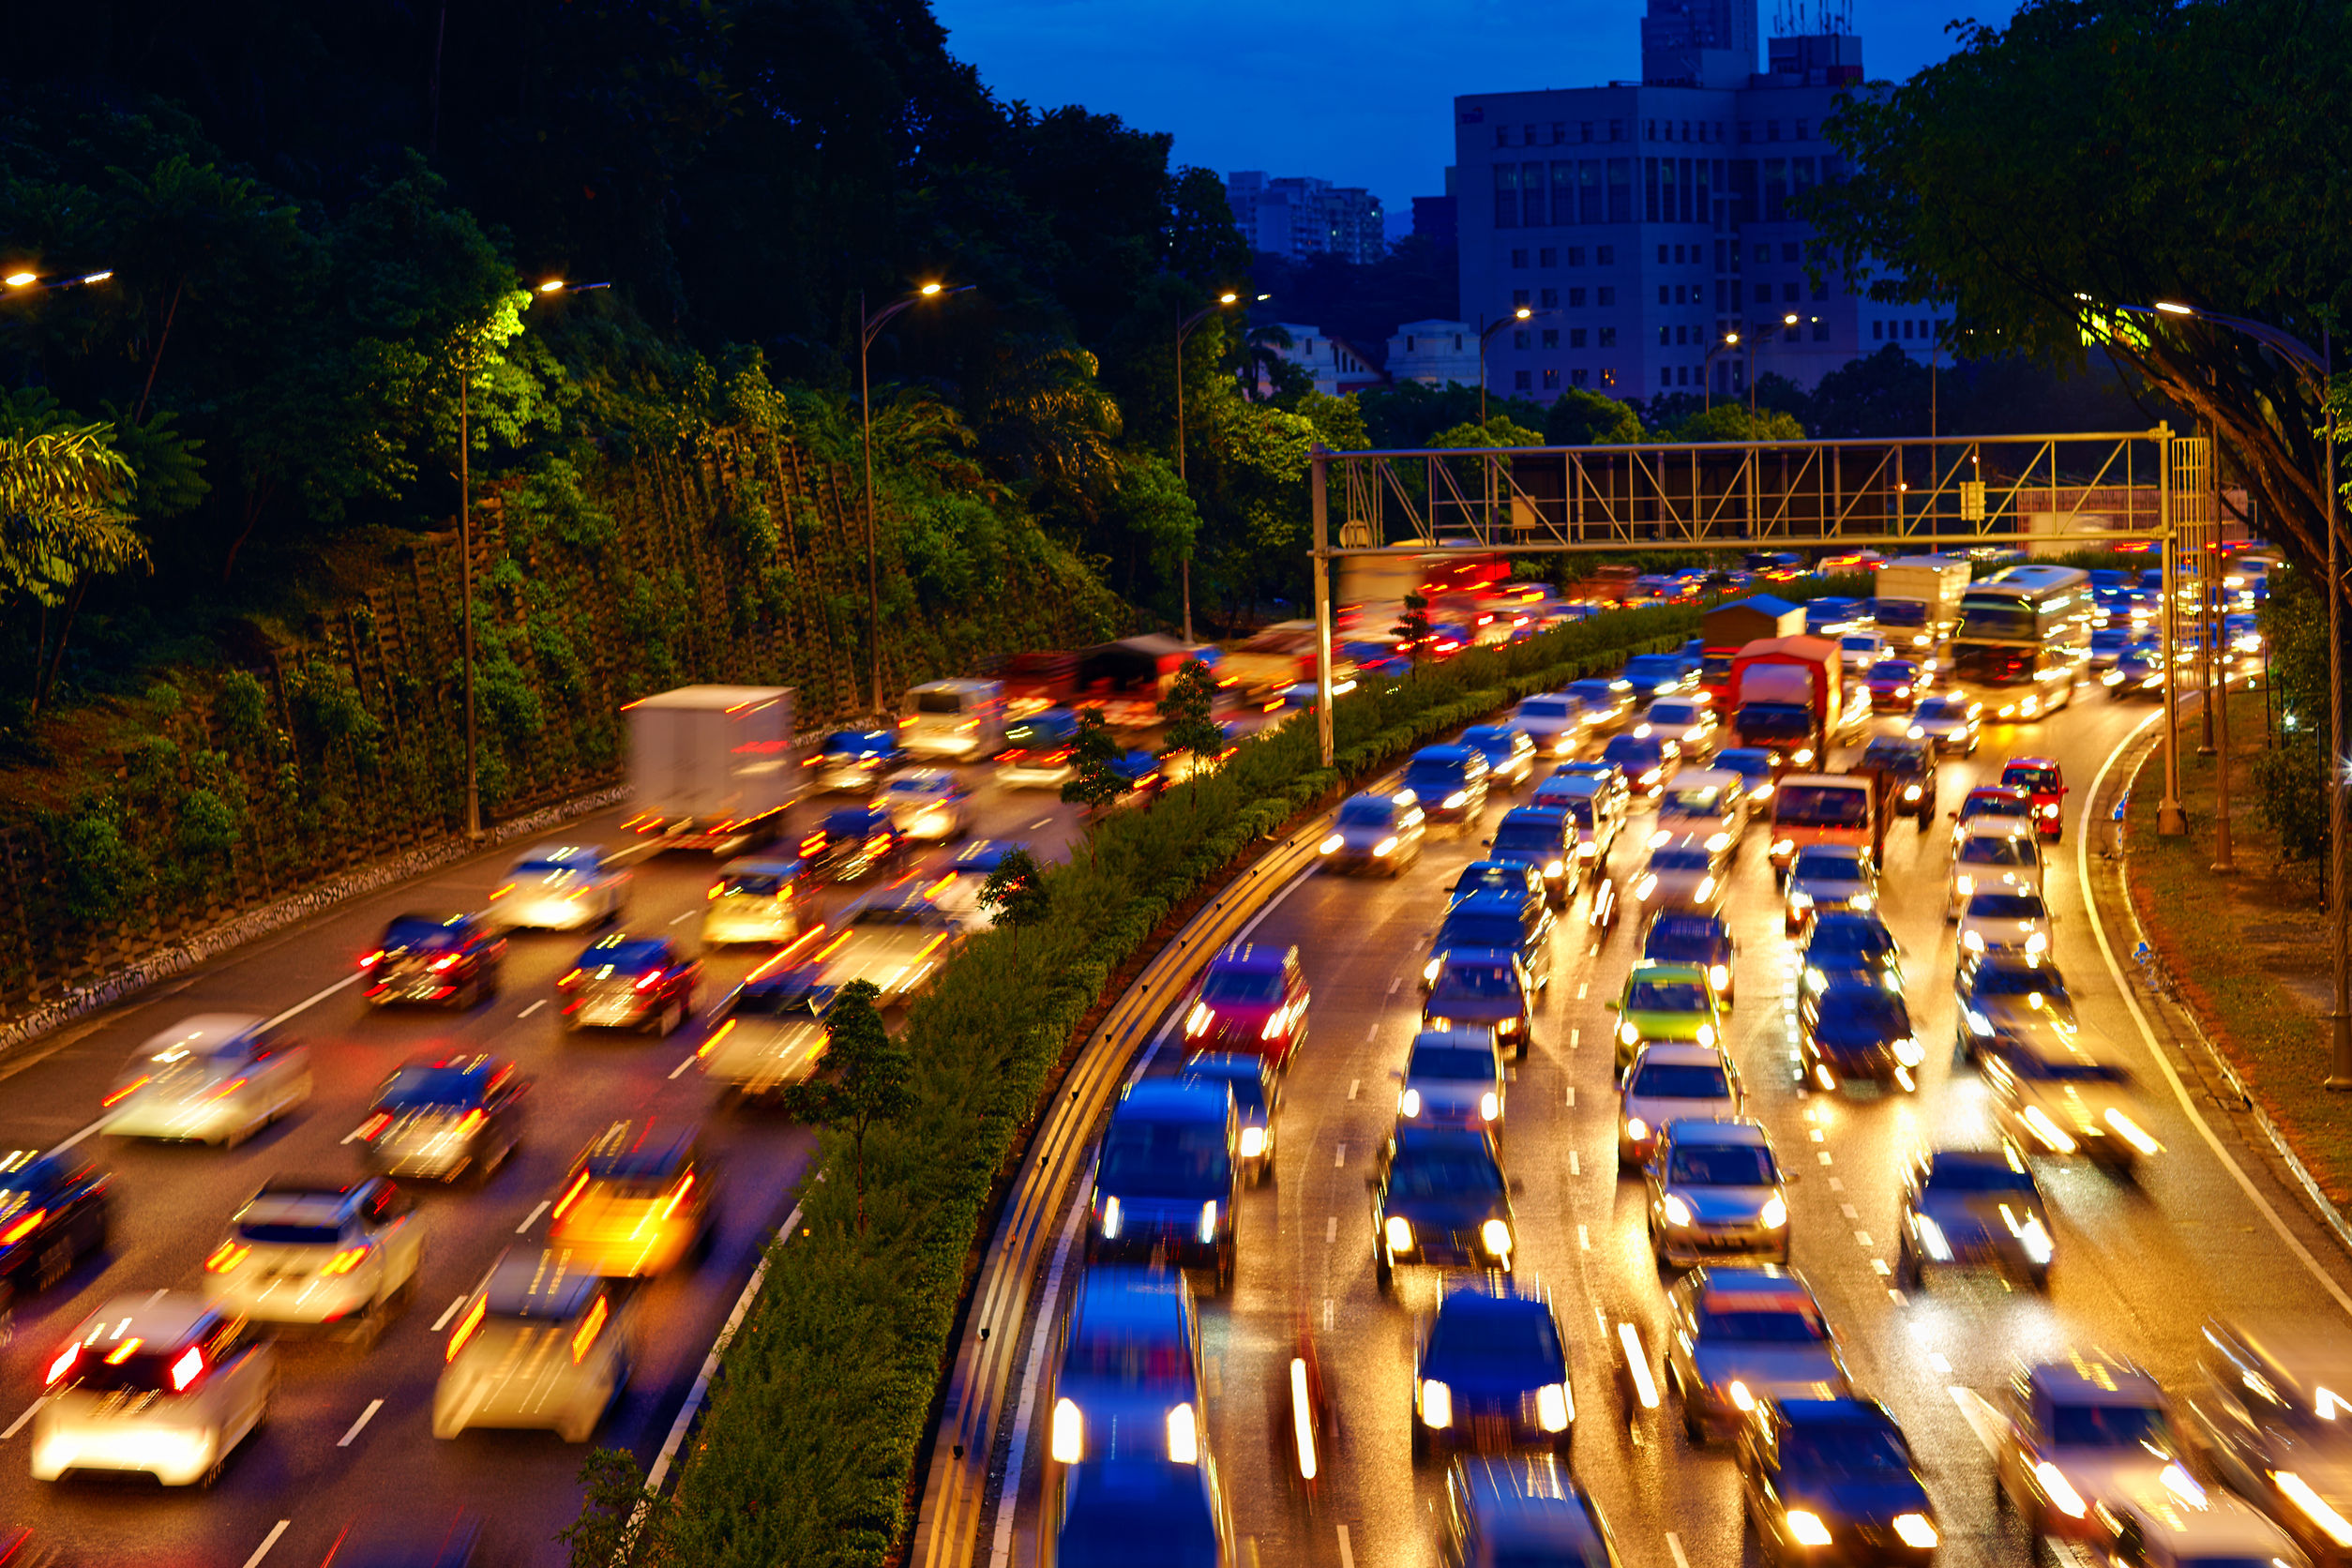
\includegraphics[width=\textwidth, clip, trim={0 100 0 150}]{title.jpg}}
\institute{\textbf{Cranfield University}}
\date{June 13, 2019}
%\setbeamercovered{transparent}
%\setbeamertemplate{navigation symbols}{}
\begin{document}
	\maketitle
	\begin{frame}
		\frametitle{Contents Slide}
		\tableofcontents{}
	\end{frame}
	
\section{Main Aims and Challenges}
	\begin{frame}
		\frametitle{Main Aims and Challenges}
		Main aims:
		\begin{itemize}
		    \item To develop a traffic flow modelling tool 
		    \item Capability of modelling complicated road networks
		    \item Numerically solving a governing PDE using various methods/tools from CFD
		\end{itemize}
		\vspace{0.5cm}
		Challenges:
		\begin{itemize}
		    \item How can you unambiguously describe a traffic network as input for a computer program?
		    \item Coupling a \emph{numerical} PDE solver with a \emph{probabilistic} method for governing flow through junctions
		    \begin{itemize}
		        \item Interaction of junction boundary information on incoming and outgoing roads
		    \end{itemize}
		\end{itemize}
	\end{frame}
	
\section{Research Objectives}
	\begin{frame}
		\frametitle{Research Objectives}
		By addressing the previous aims and challenges, the following can be achieved:
		\begin{itemize}
		    \item Assess the influence of numerical methods on microscale decisions relevant to applied problems
			\item Design a suitable test case to expose advantages and disadvantages in network traffic flow solvers 
			\item Calibrate the model using empirical data on real roads
		\end{itemize}
	\end{frame}
	
\section{Methodology}
	\begin{frame}
		\frametitle{Methodologies}
		Existing methodologies:
		\begin{itemize}
		    \item Microscopic - modelling individual cars
		    \item Macroscopic - aggregate variables for density $\rho$, flow rate $f$, velocity $u$
		\end{itemize}
		\vspace{0.5cm}
		My method:
		\begin{itemize}
			\item A Godunov numerical solver for the macroscopic Lighthill, Whitham, Richards (1955/56) conservation model: $$\frac{\partial\rho}{\partial t}+\frac{\partial f}{\partial x}=0$$
			\item Traffic distribution matrix (TDM) (Shi-Guo, 2016) determines the flow decisions at junctions
		\end{itemize}
	\end{frame}
	
	\begin{frame}{Traffic Distribution Matrix}
	TDM elements, $A=(a_{ij})$, describe the proportion of traffic passing through a junction from incoming road $i$ to outgoing road $j$,
	\begin{equation*}
    	A = 
    	\begin{pmatrix}
    	    a_{1,1} & a_{1,2} & \cdots & a_{1,n} \\
    	    a_{2,1} & a_{2,2} & \cdots & a_{2,n} \\
    	    \vdots  & \vdots  & \ddots & \vdots  \\
    	    a_{m,1} & a_{m,2} & \cdots & a_{m,n}
    	\end{pmatrix}
	\end{equation*}
	\centering
	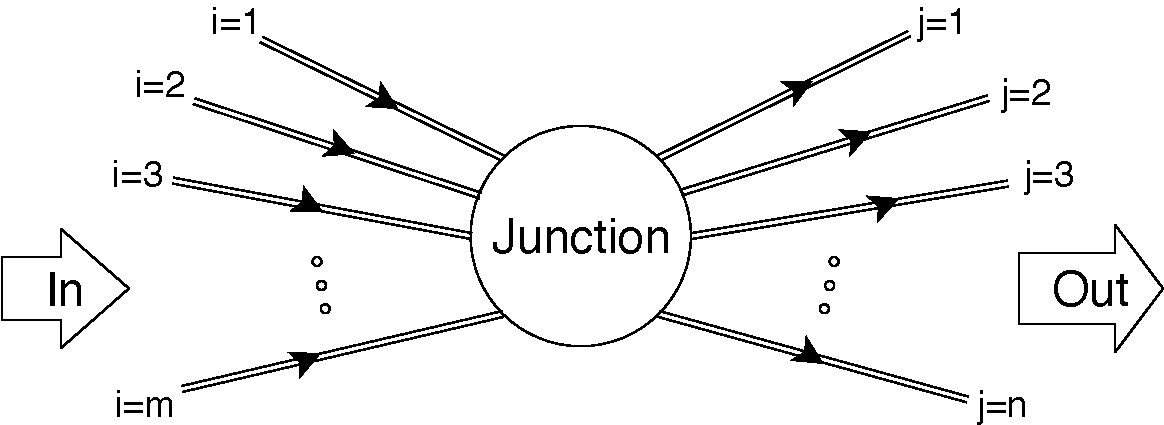
\includegraphics[width=0.9\textwidth]{junction.pdf}
	\end{frame}
	
\section{Preliminary Simulation}
	\begin{frame}
		\frametitle{Preliminary Simulation}
		\begin{itemize}
		    \item Simple network of a 1-2 split exercising a preferred route by the traffic distribution matrix (play movie)
		    $$A=[a_{1,1},\,a_{1,2}]=[0.7,\,0.3]$$
		\end{itemize}
		\vspace{0.5cm}
		\centering
		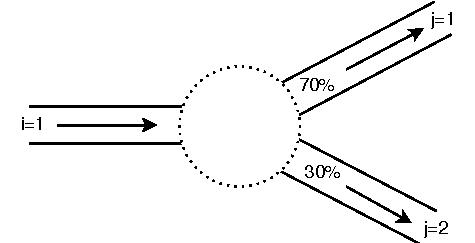
\includegraphics[width=0.5\textwidth]{1to2.pdf}
	\end{frame}
	
\section{Future Work}
	\begin{frame}
		\frametitle{Future Work}
		Next steps:
		\begin{itemize}
		    \item Expand the capabilities and behaviour of the current program:
		    \begin{itemize}
		        \item Junctions of $m$-incoming and $n$-outgoing roads
		        \item Network of many junctions
		        \item Introduce an input file for quicker test simulations of varying parameters ($\delta x$, $CFL$, etc.)
		        \item Add extra numerical method options: discretisation, gradient limiters, reconstruction
		    \end{itemize}
		    \item Verify the numerical methods against test cases in current papers
		\end{itemize}
	\end{frame}

\end{document}